\documentclass{article}\usepackage[]{graphicx}\usepackage[]{color}
%% maxwidth is the original width if it is less than linewidth
%% otherwise use linewidth (to make sure the graphics do not exceed the margin)
\makeatletter
\def\maxwidth{ %
  \ifdim\Gin@nat@width>\linewidth
    \linewidth
  \else
    \Gin@nat@width
  \fi
}
\makeatother

\definecolor{fgcolor}{rgb}{0.345, 0.345, 0.345}
\newcommand{\hlnum}[1]{\textcolor[rgb]{0.686,0.059,0.569}{#1}}%
\newcommand{\hlstr}[1]{\textcolor[rgb]{0.192,0.494,0.8}{#1}}%
\newcommand{\hlcom}[1]{\textcolor[rgb]{0.678,0.584,0.686}{\textit{#1}}}%
\newcommand{\hlopt}[1]{\textcolor[rgb]{0,0,0}{#1}}%
\newcommand{\hlstd}[1]{\textcolor[rgb]{0.345,0.345,0.345}{#1}}%
\newcommand{\hlkwa}[1]{\textcolor[rgb]{0.161,0.373,0.58}{\textbf{#1}}}%
\newcommand{\hlkwb}[1]{\textcolor[rgb]{0.69,0.353,0.396}{#1}}%
\newcommand{\hlkwc}[1]{\textcolor[rgb]{0.333,0.667,0.333}{#1}}%
\newcommand{\hlkwd}[1]{\textcolor[rgb]{0.737,0.353,0.396}{\textbf{#1}}}%

\usepackage{framed}
\makeatletter
\newenvironment{kframe}{%
 \def\at@end@of@kframe{}%
 \ifinner\ifhmode%
  \def\at@end@of@kframe{\end{minipage}}%
  \begin{minipage}{\columnwidth}%
 \fi\fi%
 \def\FrameCommand##1{\hskip\@totalleftmargin \hskip-\fboxsep
 \colorbox{shadecolor}{##1}\hskip-\fboxsep
     % There is no \\@totalrightmargin, so:
     \hskip-\linewidth \hskip-\@totalleftmargin \hskip\columnwidth}%
 \MakeFramed {\advance\hsize-\width
   \@totalleftmargin\z@ \linewidth\hsize
   \@setminipage}}%
 {\par\unskip\endMakeFramed%
 \at@end@of@kframe}
\makeatother

\definecolor{shadecolor}{rgb}{.97, .97, .97}
\definecolor{messagecolor}{rgb}{0, 0, 0}
\definecolor{warningcolor}{rgb}{1, 0, 1}
\definecolor{errorcolor}{rgb}{1, 0, 0}
\newenvironment{knitrout}{}{} % an empty environment to be redefined in TeX

\usepackage{alltt}
\IfFileExists{upquote.sty}{\usepackage{upquote}}{}
\begin{document}






\begin{knitrout}
\definecolor{shadecolor}{rgb}{0.969, 0.969, 0.969}\color{fgcolor}\begin{kframe}
\begin{alltt}
\hlkwd{setPar}\hlstd{()}
\hlkwd{plot}\hlstd{(SelByYear,} \hlkwc{x}\hlstd{=}\hlnum{2006}\hlopt{:}\hlnum{2015}\hlstd{,} \hlkwc{ylim}\hlstd{=}\hlkwd{c}\hlstd{(}\hlkwd{min}\hlstd{( CISelByYear),} \hlkwd{max}\hlstd{( CISelByYear)),} \hlkwc{xlab}\hlstd{=}\hlstr{"Year"}\hlstd{,} \hlkwc{ylab} \hlstd{=} \hlstr{"Selection gradient"}\hlstd{,} \hlkwc{main} \hlstd{=} \hlstr{"\textbackslash{}\textbackslash{}textbf\{(A)\} Total selection"}\hlstd{)}
\hlkwd{abline}\hlstd{(}\hlkwc{h}\hlstd{=}\hlnum{0}\hlstd{)}
\hlkwd{arrows}\hlstd{(}\hlkwc{x0} \hlstd{=} \hlnum{2006}\hlopt{:}\hlnum{2015}\hlstd{,}\hlkwc{x1} \hlstd{=} \hlnum{2006}\hlopt{:}\hlnum{2015}\hlstd{,}\hlkwc{code} \hlstd{=} \hlnum{3}\hlstd{,} \hlkwc{y0} \hlstd{= CISelByYear[}\hlnum{1}\hlstd{,],}
       \hlkwc{y1} \hlstd{= CISelByYear[}\hlnum{2}\hlstd{,],} \hlkwc{angle} \hlstd{=} \hlnum{90}\hlstd{,}\hlkwc{length} \hlstd{=} \hlnum{0.1}\hlstd{)}
\hlstd{m0all} \hlkwb{<-} \hlkwd{glm}\hlstd{(Fitness} \hlopt{~} \hlnum{1} \hlopt{+} \hlstd{StMass} \hlopt{+} \hlstd{Sex} \hlopt{+}\hlstd{Age ,} \hlkwc{data}\hlstd{=YearPheno,} \hlkwc{family}\hlstd{=poisson)}
\hlkwd{abline}\hlstd{(}\hlkwc{h}\hlstd{=}\hlkwd{coefficients}\hlstd{(m0all)[}\hlnum{2}\hlstd{],} \hlkwc{lty}\hlstd{=}\hlnum{2}\hlstd{,} \hlkwc{lwd}\hlstd{=}\hlnum{5}\hlstd{)}
\hlstd{sm0all} \hlkwb{<-} \hlkwd{summary}\hlstd{(m0all)}
\hlstd{lowm0all} \hlkwb{<-} \hlkwd{coefficients}\hlstd{(m0all)[}\hlnum{2}\hlstd{]}\hlopt{+}\hlnum{1.96}\hlopt{*}\hlstd{sm0all}\hlopt{$}\hlstd{coefficients[}\hlnum{2}\hlstd{,}\hlnum{2}\hlstd{]}
\hlstd{highm0all} \hlkwb{<-} \hlkwd{coefficients}\hlstd{(m0all)[}\hlnum{2}\hlstd{]}\hlopt{-}\hlnum{1.96}\hlopt{*}\hlstd{sm0all}\hlopt{$}\hlstd{coefficients[}\hlnum{2}\hlstd{,}\hlnum{2}\hlstd{]}
\hlkwd{polygon}\hlstd{(}\hlkwc{x}\hlstd{=}\hlkwd{c}\hlstd{(}\hlnum{2005}\hlstd{,}\hlnum{2016}\hlstd{,}\hlnum{2016}\hlstd{,}\hlnum{2005}\hlstd{),}\hlkwc{y}\hlstd{=}\hlkwd{c}\hlstd{(lowm0all,lowm0all, highm0all, highm0all),}
        \hlkwc{fillOddEven} \hlstd{=} \hlnum{TRUE}\hlstd{,} \hlkwc{col}\hlstd{=}\hlkwd{rgb}\hlstd{(}\hlnum{0.1}\hlstd{,}\hlnum{0.1}\hlstd{,}\hlnum{0.1}\hlstd{,}\hlnum{0.3}\hlstd{),} \hlkwc{lty}\hlstd{=}\hlnum{2}\hlstd{)}
\end{alltt}
\end{kframe}
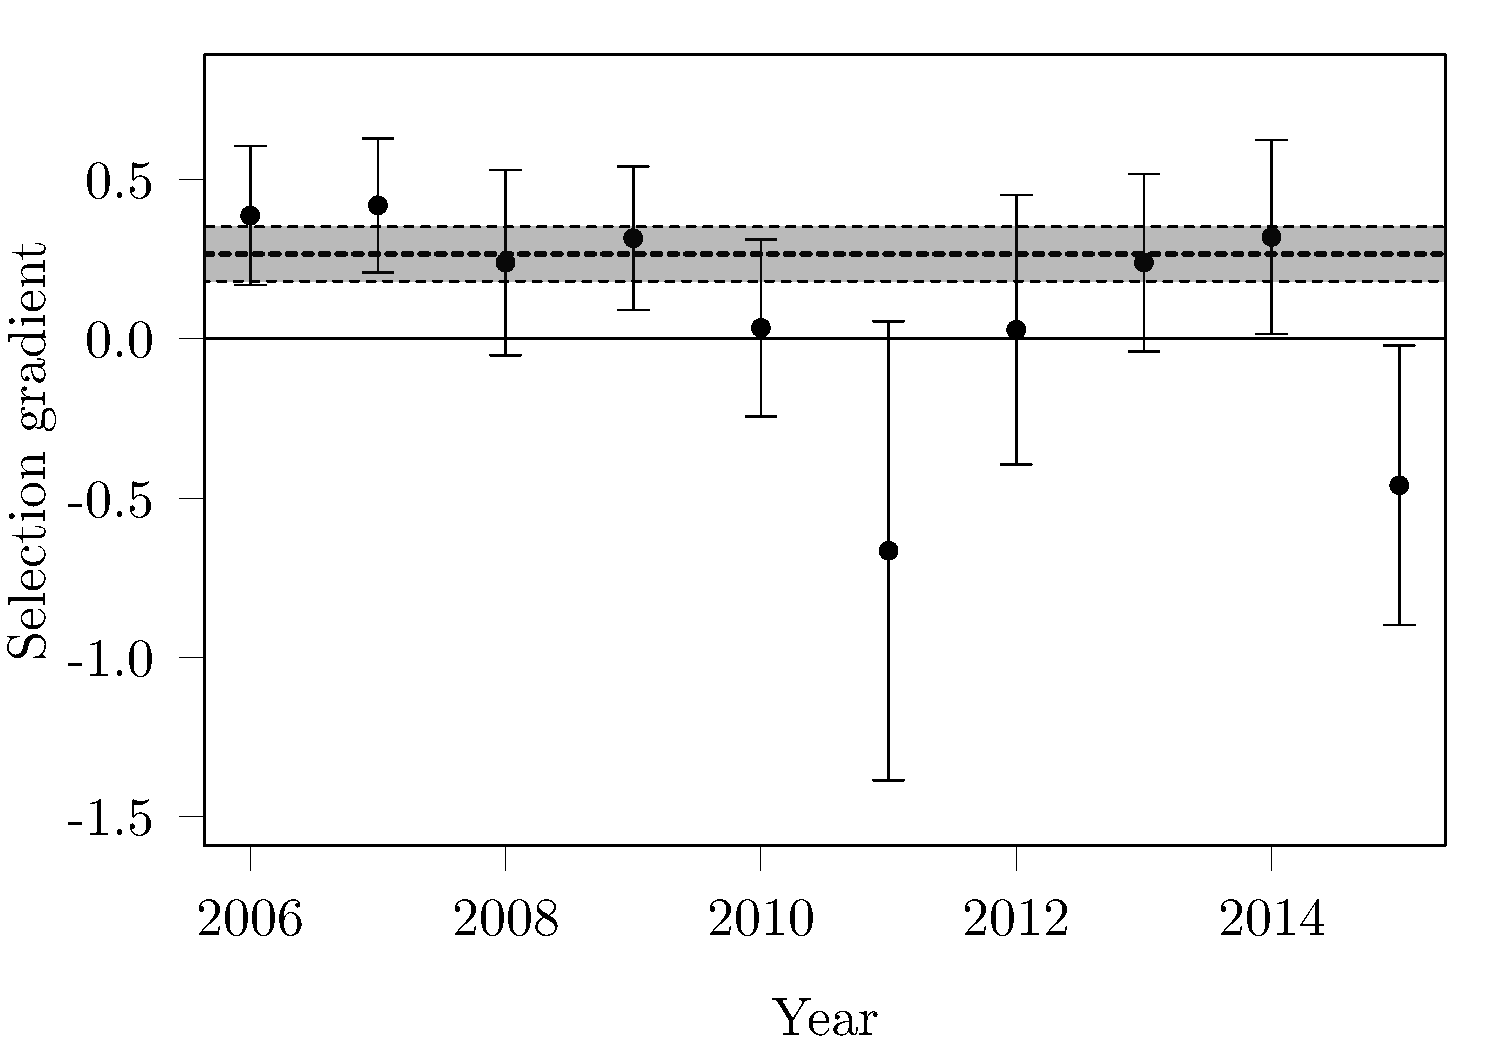
\includegraphics[width=\maxwidth]{figure/SelByYear-1} 
\begin{kframe}\begin{alltt}
\hlcom{#points(x=2006:2015,y=unlist(coefficients(mmRnoCorfitness)$Year["StMass"]), pch=17)}
\end{alltt}
\end{kframe}
\end{knitrout}

\begin{knitrout}
\definecolor{shadecolor}{rgb}{0.969, 0.969, 0.969}\color{fgcolor}\begin{kframe}
\begin{alltt}
\hlkwd{setPar}\hlstd{()}
\hlkwd{plot}\hlstd{(SelByYearRho,} \hlkwc{x}\hlstd{=}\hlnum{2006}\hlopt{:}\hlnum{2015}\hlstd{,} \hlkwc{ylim}\hlstd{=}\hlkwd{c}\hlstd{(}\hlkwd{min}\hlstd{( CISelByYearRho),} \hlkwd{max}\hlstd{( CISelByYearRho)),} \hlkwc{xlab}\hlstd{=}\hlstr{"Year"}\hlstd{,} \hlkwc{ylab} \hlstd{=} \hlstr{"Selection gradient on $\textbackslash{}\textbackslash{}rho$"}\hlstd{,} \hlkwc{main} \hlstd{=} \hlstr{"\textbackslash{}\textbackslash{}textbf\{(B)\} Fertility selection"}\hlstd{)}
\hlkwd{abline}\hlstd{(}\hlkwc{h}\hlstd{=}\hlnum{0}\hlstd{)}
\hlkwd{sd}\hlstd{(SelByYearRho)}
\end{alltt}
\begin{verbatim}
## [1] 0.3521055
\end{verbatim}
\begin{alltt}
\hlkwd{arrows}\hlstd{(}\hlkwc{x0} \hlstd{=} \hlnum{2006}\hlopt{:}\hlnum{2015}\hlstd{,}\hlkwc{x1} \hlstd{=} \hlnum{2006}\hlopt{:}\hlnum{2015}\hlstd{,}\hlkwc{code} \hlstd{=} \hlnum{3}\hlstd{,} \hlkwc{y0} \hlstd{= CISelByYearRho[}\hlnum{1}\hlstd{,],}
       \hlkwc{y1} \hlstd{= CISelByYearRho[}\hlnum{2}\hlstd{,],} \hlkwc{angle} \hlstd{=} \hlnum{90}\hlstd{,}\hlkwc{length} \hlstd{=} \hlnum{0.1}\hlstd{)}
\hlstd{m0allRho} \hlkwb{<-} \hlkwd{glm}\hlstd{(Rho} \hlopt{~} \hlnum{1} \hlopt{+} \hlstd{StMass} \hlopt{+} \hlstd{Sex ,} \hlkwc{data}\hlstd{=YearPheno[YearPheno}\hlopt{$}\hlstd{Age}\hlopt{==}\hlstr{"A"}\hlstd{,],} \hlkwc{family}\hlstd{=quasipoisson)}
\hlkwd{abline}\hlstd{(}\hlkwc{h}\hlstd{=}\hlkwd{coefficients}\hlstd{(m0allRho)[}\hlnum{2}\hlstd{],} \hlkwc{lty}\hlstd{=}\hlnum{2}\hlstd{)}
\hlstd{sm0allRho} \hlkwb{<-} \hlkwd{summary}\hlstd{(m0allRho)}
\hlstd{lowm0allRho} \hlkwb{<-} \hlkwd{coefficients}\hlstd{(m0allRho)[}\hlnum{2}\hlstd{]}\hlopt{+}\hlnum{1.96}\hlopt{*}\hlstd{sm0allRho}\hlopt{$}\hlstd{coefficients[}\hlnum{2}\hlstd{,}\hlnum{2}\hlstd{]}
\hlstd{highm0allRho} \hlkwb{<-} \hlkwd{coefficients}\hlstd{(m0allRho)[}\hlnum{2}\hlstd{]}\hlopt{-}\hlnum{1.96}\hlopt{*}\hlstd{sm0allRho}\hlopt{$}\hlstd{coefficients[}\hlnum{2}\hlstd{,}\hlnum{2}\hlstd{]}
\hlkwd{polygon}\hlstd{(}\hlkwc{x}\hlstd{=}\hlkwd{c}\hlstd{(}\hlnum{2005}\hlstd{,}\hlnum{2016}\hlstd{,}\hlnum{2016}\hlstd{,}\hlnum{2005}\hlstd{),}\hlkwc{y}\hlstd{=}\hlkwd{c}\hlstd{(lowm0allRho,lowm0allRho, highm0allRho, highm0allRho),}
        \hlkwc{fillOddEven} \hlstd{=} \hlnum{TRUE}\hlstd{,} \hlkwc{col}\hlstd{=}\hlkwd{rgb}\hlstd{(}\hlnum{0.1}\hlstd{,}\hlnum{0.1}\hlstd{,}\hlnum{0.1}\hlstd{,}\hlnum{0.5}\hlstd{),} \hlkwc{lty}\hlstd{=}\hlnum{2}\hlstd{)}
\end{alltt}
\end{kframe}
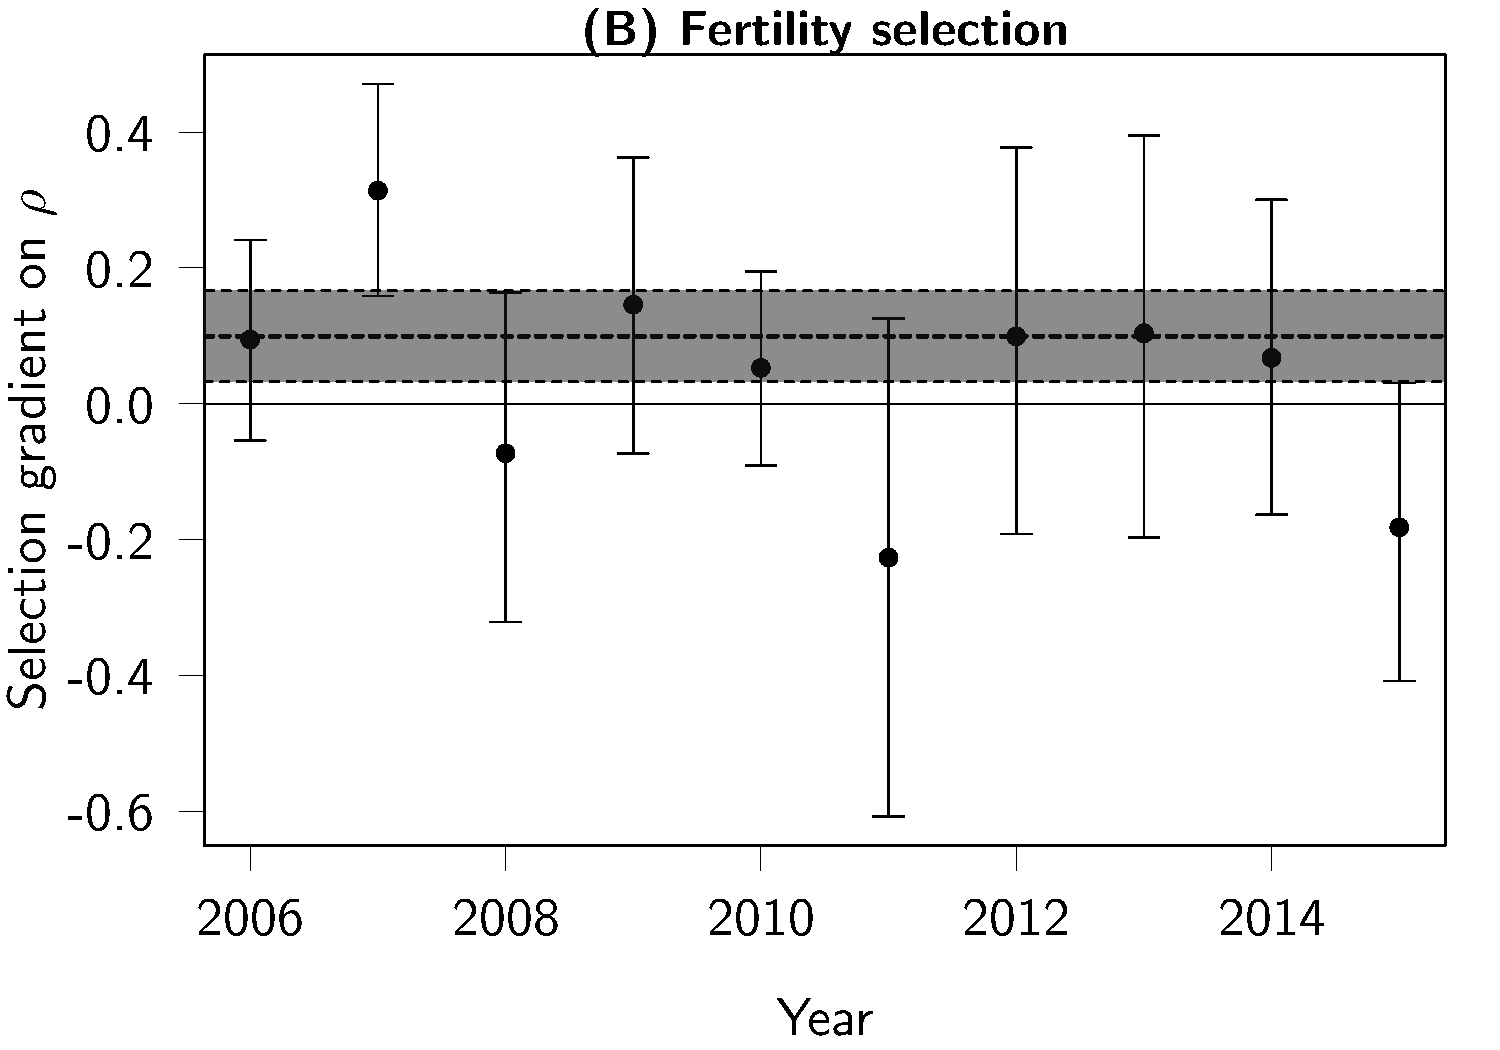
\includegraphics[width=\maxwidth]{figure/SelByYearRho-1} 

\end{knitrout}


\begin{knitrout}
\definecolor{shadecolor}{rgb}{0.969, 0.969, 0.969}\color{fgcolor}\begin{kframe}
\begin{alltt}
\hlkwd{setPar}\hlstd{()}
\hlkwd{plot}\hlstd{(SelByYearPhi,} \hlkwc{x}\hlstd{=}\hlnum{2006}\hlopt{:}\hlnum{2015}\hlstd{,} \hlkwc{ylim}\hlstd{=}\hlkwd{c}\hlstd{(}\hlkwd{min}\hlstd{( CISelByYearPhi,} \hlkwc{na.rm}\hlstd{=}\hlnum{TRUE}\hlstd{),} \hlkwd{max}\hlstd{( CISelByYearPhi,} \hlkwc{na.rm}\hlstd{=}\hlnum{TRUE}\hlstd{)),} \hlkwc{xlab}\hlstd{=}\hlstr{"Year"}\hlstd{,} \hlkwc{ylab} \hlstd{=} \hlstr{"Selection gradient on $\textbackslash{}\textbackslash{}phi$"}\hlstd{,} \hlkwc{main} \hlstd{=} \hlstr{"\textbackslash{}\textbackslash{}textbf\{(C)\} Viability selection"}\hlstd{)}
\hlkwd{abline}\hlstd{(}\hlkwc{h}\hlstd{=}\hlnum{0}\hlstd{)}
\hlkwd{arrows}\hlstd{(}\hlkwc{x0} \hlstd{=} \hlnum{2006}\hlopt{:}\hlnum{2015}\hlstd{,}\hlkwc{x1} \hlstd{=} \hlnum{2006}\hlopt{:}\hlnum{2015}\hlstd{,}\hlkwc{code} \hlstd{=} \hlnum{3}\hlstd{,} \hlkwc{y0} \hlstd{= CISelByYearPhi[}\hlnum{1}\hlstd{,],}
       \hlkwc{y1} \hlstd{= CISelByYearPhi[}\hlnum{2}\hlstd{,],} \hlkwc{angle} \hlstd{=} \hlnum{90}\hlstd{,}\hlkwc{length} \hlstd{=} \hlnum{0.1}\hlstd{)}
\hlstd{m0allphi} \hlkwb{<-} \hlkwd{glm}\hlstd{(Phi} \hlopt{~} \hlnum{1} \hlopt{+} \hlstd{StMass} \hlopt{+} \hlstd{Sex} \hlopt{+}\hlstd{Age ,} \hlkwc{data}\hlstd{=YearPheno[YearPheno}\hlopt{$}\hlstd{Year}\hlopt{<}\hlnum{2015}\hlstd{,],} \hlkwc{family}\hlstd{=binomial)}
\hlkwd{abline}\hlstd{(}\hlkwc{h}\hlstd{=}\hlkwd{coefficients}\hlstd{(m0allphi)[}\hlnum{2}\hlstd{],} \hlkwc{lty}\hlstd{=}\hlnum{2}\hlstd{)}
\hlstd{sm0allphi} \hlkwb{<-} \hlkwd{summary}\hlstd{(m0allphi)}
\hlstd{lowm0allphi} \hlkwb{<-} \hlkwd{coefficients}\hlstd{(m0allphi)[}\hlnum{2}\hlstd{]}\hlopt{+}\hlnum{1.96}\hlopt{*}\hlstd{sm0allphi}\hlopt{$}\hlstd{coefficients[}\hlnum{2}\hlstd{,}\hlnum{2}\hlstd{]}
\hlstd{highm0allphi} \hlkwb{<-} \hlkwd{coefficients}\hlstd{(m0allphi)[}\hlnum{2}\hlstd{]}\hlopt{-}\hlnum{1.96}\hlopt{*}\hlstd{sm0allphi}\hlopt{$}\hlstd{coefficients[}\hlnum{2}\hlstd{,}\hlnum{2}\hlstd{]}
\hlkwd{polygon}\hlstd{(}\hlkwc{x}\hlstd{=}\hlkwd{c}\hlstd{(}\hlnum{2005}\hlstd{,}\hlnum{2016}\hlstd{,}\hlnum{2016}\hlstd{,}\hlnum{2005}\hlstd{),}\hlkwc{y}\hlstd{=}\hlkwd{c}\hlstd{(lowm0allphi,lowm0allphi, highm0allphi, highm0allphi),}
        \hlkwc{fillOddEven} \hlstd{=} \hlnum{TRUE}\hlstd{,} \hlkwc{col}\hlstd{=}\hlkwd{rgb}\hlstd{(}\hlnum{0.1}\hlstd{,}\hlnum{0.1}\hlstd{,}\hlnum{0.1}\hlstd{,}\hlnum{0.5}\hlstd{),} \hlkwc{lty}\hlstd{=}\hlnum{2} \hlstd{)}
\end{alltt}
\end{kframe}
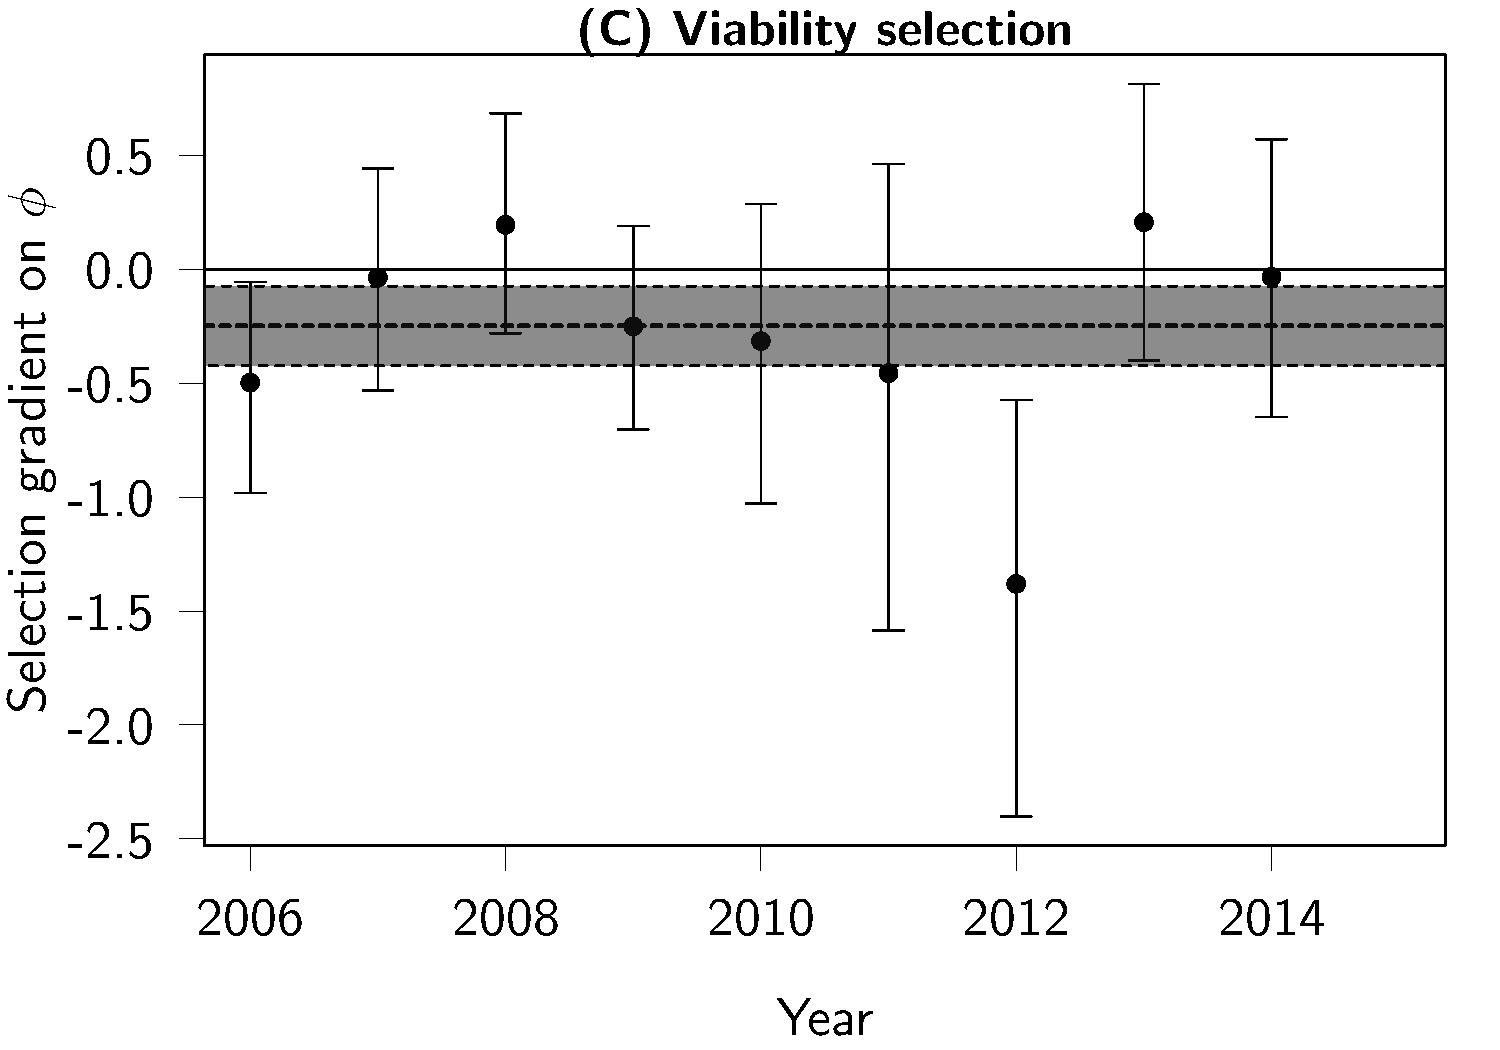
\includegraphics[width=\maxwidth]{figure/SelByYearPhi-1} 

\end{knitrout}
Correlation fertility viability
\begin{knitrout}
\definecolor{shadecolor}{rgb}{0.969, 0.969, 0.969}\color{fgcolor}\begin{kframe}
\begin{alltt}
\hlkwd{cor.test}\hlstd{(YearPheno}\hlopt{$}\hlstd{Phi,YearPheno}\hlopt{$}\hlstd{Rho)}
\end{alltt}
\begin{verbatim}
## 
## 	Pearson's product-moment correlation
## 
## data:  YearPheno$Phi and YearPheno$Rho
## t = -1.9473, df = 1292, p-value = 0.05171
## alternative hypothesis: true correlation is not equal to 0
## 95 percent confidence interval:
##  -0.1082724891  0.0003989614
## sample estimates:
##         cor 
## -0.05409695
\end{verbatim}
\end{kframe}
\end{knitrout}

\begin{knitrout}
\definecolor{shadecolor}{rgb}{0.969, 0.969, 0.969}\color{fgcolor}\begin{kframe}
\begin{alltt}
\hlkwd{sd}\hlstd{(SelByYear)}
\end{alltt}
\begin{verbatim}
## [1] 0.3689205
\end{verbatim}
\begin{alltt}
\hlkwd{coefficients}\hlstd{(m0all)[}\hlnum{2}\hlstd{]}
\end{alltt}
\begin{verbatim}
##    StMass 
## 0.2663751
\end{verbatim}
\begin{alltt}
\hlkwd{mean}\hlstd{(SeSelByYear)}
\end{alltt}
\begin{verbatim}
## [1] 0.2129145
\end{verbatim}
\begin{alltt}
\hlstd{sm0all}
\end{alltt}
\begin{verbatim}
## 
## Call:
## glm(formula = Fitness ~ 1 + StMass + Sex + Age, family = poisson, 
##     data = YearPheno)
## 
## Deviance Residuals: 
##     Min       1Q   Median       3Q      Max  
## -3.0411  -1.0989  -0.9829   0.8946   4.6194  
## 
## Coefficients:
##             Estimate Std. Error z value Pr(>|z|)    
## (Intercept)  0.80415    0.05341  15.055  < 2e-16 ***
## StMass       0.26638    0.04373   6.091 1.12e-09 ***
## SexMale     -0.06913    0.04788  -1.444    0.149    
## AgeJ        -1.15530    0.09571 -12.070  < 2e-16 ***
## ---
## Signif. codes:  0 '***' 0.001 '**' 0.01 '*' 0.05 '.' 0.1 ' ' 1
## 
## (Dispersion parameter for poisson family taken to be 1)
## 
##     Null deviance: 3572.2  on 1267  degrees of freedom
## Residual deviance: 2440.6  on 1264  degrees of freedom
##   (26 observations deleted due to missingness)
## AIC: 4220.8
## 
## Number of Fisher Scoring iterations: 6
\end{verbatim}
\begin{alltt}
\hlstd{sm0allRho}
\end{alltt}
\begin{verbatim}
## 
## Call:
## glm(formula = Rho ~ 1 + StMass + Sex, family = quasipoisson, 
##     data = YearPheno[YearPheno$Age == "A", ])
## 
## Deviance Residuals: 
##     Min       1Q   Median       3Q      Max  
## -2.8900  -1.4039  -0.2919   0.7730   4.5874  
## 
## Coefficients:
##             Estimate Std. Error t value Pr(>|t|)    
## (Intercept)  0.68281    0.09383   7.277 1.26e-12 ***
## StMass       0.16722    0.08068   2.073  0.03868 *  
## SexMale      0.24668    0.08763   2.815  0.00506 ** 
## ---
## Signif. codes:  0 '***' 0.001 '**' 0.01 '*' 0.05 '.' 0.1 ' ' 1
## 
## (Dispersion parameter for quasipoisson family taken to be 2.352076)
## 
##     Null deviance: 1337.4  on 524  degrees of freedom
## Residual deviance: 1295.7  on 522  degrees of freedom
##   (5 observations deleted due to missingness)
## AIC: NA
## 
## Number of Fisher Scoring iterations: 5
\end{verbatim}
\begin{alltt}
\hlstd{sm0allphi}
\end{alltt}
\begin{verbatim}
## 
## Call:
## glm(formula = Phi ~ 1 + StMass + Sex + Age, family = binomial, 
##     data = YearPheno[YearPheno$Year < 2015, ])
## 
## Deviance Residuals: 
##     Min       1Q   Median       3Q      Max  
## -1.2431  -0.7023  -0.5990  -0.3750   2.3352  
## 
## Coefficients:
##             Estimate Std. Error z value Pr(>|z|)    
## (Intercept)  -1.8261     0.2011  -9.080  < 2e-16 ***
## StMass        0.4107     0.1453   2.827   0.0047 ** 
## SexMale      -1.0712     0.1534  -6.983 2.90e-12 ***
## AgeJ          1.7408     0.2995   5.812 6.16e-09 ***
## ---
## Signif. codes:  0 '***' 0.001 '**' 0.01 '*' 0.05 '.' 0.1 ' ' 1
## 
## (Dispersion parameter for binomial family taken to be 1)
## 
##     Null deviance: 1256.4  on 1150  degrees of freedom
## Residual deviance: 1165.5  on 1147  degrees of freedom
##   (26 observations deleted due to missingness)
## AIC: 1173.5
## 
## Number of Fisher Scoring iterations: 4
\end{verbatim}
\begin{alltt}
\hlkwd{sd}\hlstd{(SelByYearPhi,}\hlkwc{na.rm}\hlstd{=T)}
\end{alltt}
\begin{verbatim}
## [1] 0.6993909
\end{verbatim}
\begin{alltt}
\hlkwd{mean}\hlstd{(SeSelByYearPhi,}\hlkwc{na.rm}\hlstd{=T)}
\end{alltt}
\begin{verbatim}
## [1] 0.5589321
\end{verbatim}
\begin{alltt}
\hlkwd{sd}\hlstd{(SelByYearRho)}
\end{alltt}
\begin{verbatim}
## [1] 0.3521055
\end{verbatim}
\begin{alltt}
\hlkwd{mean}\hlstd{(SeSelByYearRho)}
\end{alltt}
\begin{verbatim}
## [1] 0.2741972
\end{verbatim}
\end{kframe}
\end{knitrout}

Test of fluctuation of selection on fitness.
\begin{knitrout}
\definecolor{shadecolor}{rgb}{0.969, 0.969, 0.969}\color{fgcolor}\begin{kframe}
\begin{alltt}
\hlkwd{summary}\hlstd{(mmRnoCorfitness)}
\end{alltt}
\begin{verbatim}
## Generalized linear mixed model fit by maximum likelihood (Laplace
##   Approximation) [glmerMod]
##  Family: poisson  ( log )
## Formula: Fitness ~ 1 + StMass + Sex + Age + (1 | Year) + (0 + StMass |  
##     Year)
##    Data: YearPheno[!is.na(YearPheno$StMass), ]
## 
##      AIC      BIC   logLik deviance df.resid 
##   3984.6   4015.5  -1986.3   3972.6     1262 
## 
## Scaled residuals: 
##     Min      1Q  Median      3Q     Max 
## -2.3621 -0.8015 -0.6154  0.9164  5.0348 
## 
## Random effects:
##  Groups Name        Variance Std.Dev.
##  Year   (Intercept) 0.1762   0.4198  
##  Year.1 StMass      0.0143   0.1196  
## Number of obs: 1268, groups:  Year, 10
## 
## Fixed effects:
##             Estimate Std. Error z value Pr(>|z|)    
## (Intercept)  0.79743    0.14423   5.529 3.22e-08 ***
## StMass       0.19656    0.06118   3.213  0.00132 ** 
## SexMale     -0.08054    0.04868  -1.655  0.09802 .  
## AgeJ        -1.32185    0.09794 -13.496  < 2e-16 ***
## ---
## Signif. codes:  0 '***' 0.001 '**' 0.01 '*' 0.05 '.' 0.1 ' ' 1
## 
## Correlation of Fixed Effects:
##         (Intr) StMass SexMal
## StMass  -0.243              
## SexMale -0.040 -0.208       
## AgeJ    -0.281  0.601 -0.265
\end{verbatim}
\begin{alltt}
\hlkwd{logLik}\hlstd{(mmRnoCorfitness)}
\end{alltt}
\begin{verbatim}
## 'log Lik.' -1986.296 (df=6)
\end{verbatim}
\begin{alltt}
\hlkwd{logLik}\hlstd{(mmRIfitness)}
\end{alltt}
\begin{verbatim}
## 'log Lik.' -1990.887 (df=5)
\end{verbatim}
\begin{alltt}
\hlkwd{anova}\hlstd{(mmRIfitness,mmRnoCorfitness)}
\end{alltt}
\begin{verbatim}
## Data: YearPheno[!is.na(YearPheno$StMass), ]
## Models:
## mmRIfitness: Fitness ~ 1 + StMass + Sex + Age + (1 | Year)
## mmRnoCorfitness: Fitness ~ 1 + StMass + Sex + Age + (1 | Year) + (0 + StMass | 
## mmRnoCorfitness:     Year)
##                 Df    AIC    BIC  logLik deviance  Chisq Chi Df Pr(>Chisq)
## mmRIfitness      5 3991.8 4017.5 -1990.9   3981.8                         
## mmRnoCorfitness  6 3984.6 4015.5 -1986.3   3972.6 9.1803      1   0.002446
##                   
## mmRIfitness       
## mmRnoCorfitness **
## ---
## Signif. codes:  0 '***' 0.001 '**' 0.01 '*' 0.05 '.' 0.1 ' ' 1
\end{verbatim}
\begin{alltt}
\hlstd{CImmRnoCorfitness}
\end{alltt}
\begin{verbatim}
##                   2.5 %      97.5 %
## .sig01       0.27187274  0.72057971
## .sig02       0.05109243  0.23887427
## (Intercept)  0.48613245  1.10267909
## StMass       0.06449753  0.31535917
## SexMale     -0.17634476  0.01487124
## AgeJ        -1.51480609 -1.13006779
\end{verbatim}
\begin{alltt}
\hlkwd{sqrt}\hlstd{(}\hlkwd{VarCorr}\hlstd{(mmRnoCorfitness)[[}\hlnum{2}\hlstd{]][}\hlnum{1}\hlstd{])}\hlopt{/}\hlkwd{summary}\hlstd{(mmRnoCorfitness)}\hlopt{$}\hlstd{coef[}\hlnum{2}\hlstd{,}\hlnum{1}\hlstd{]}
\end{alltt}


{\ttfamily\noindent\bfseries\color{errorcolor}{\#\# Error in eval(expr, envir, enclos): impossible de trouver la fonction "{}VarCorr"{}}}\end{kframe}
\end{knitrout}

Test of fluctuation of selection on fecundity.
\begin{knitrout}
\definecolor{shadecolor}{rgb}{0.969, 0.969, 0.969}\color{fgcolor}\begin{kframe}
\begin{alltt}
\hlkwd{summary}\hlstd{(mmRnoCorrho)}
\end{alltt}
\begin{verbatim}
## Generalized linear mixed model fit by maximum likelihood (Laplace
##   Approximation) [glmerMod]
##  Family: poisson  ( log )
## Formula: Rho ~ 1 + StMass + Sex + (1 | Year) + (0 + StMass | Year)
##    Data: YearPheno[YearPheno$Age == "A", ]
## 
##      AIC      BIC   logLik deviance df.resid 
##   2312.0   2333.3  -1151.0   2302.0      520 
## 
## Scaled residuals: 
##     Min      1Q  Median      3Q     Max 
## -2.3908 -1.0720 -0.2378  0.7582  4.8141 
## 
## Random effects:
##  Groups Name        Variance Std.Dev.
##  Year   (Intercept) 0.06270  0.2504  
##  Year.1 StMass      0.06419  0.2534  
## Number of obs: 525, groups:  Year, 10
## 
## Fixed effects:
##             Estimate Std. Error z value Pr(>|z|)    
## (Intercept)  0.71994    0.10393   6.927 4.30e-12 ***
## StMass       0.03754    0.10160   0.370    0.712    
## SexMale      0.25667    0.05869   4.373 1.23e-05 ***
## ---
## Signif. codes:  0 '***' 0.001 '**' 0.01 '*' 0.05 '.' 0.1 ' ' 1
## 
## Correlation of Fixed Effects:
##         (Intr) StMass
## StMass  -0.322       
## SexMale -0.063 -0.194
\end{verbatim}
\begin{alltt}
\hlkwd{logLik}\hlstd{(mmRnoCorrho)}
\end{alltt}
\begin{verbatim}
## 'log Lik.' -1151.002 (df=5)
\end{verbatim}
\begin{alltt}
\hlkwd{logLik}\hlstd{(mmRIrho)}
\end{alltt}
\begin{verbatim}
## 'log Lik.' -1156.07 (df=4)
\end{verbatim}
\begin{alltt}
\hlkwd{anova}\hlstd{(mmRIphi,mmRnoCorphi)}
\end{alltt}
\begin{verbatim}
## Data: YearPheno
## Models:
## mmRIphi: Phi ~ 1 + StMass + Sex + Age + (1 | Year) + (0 + StMass | Year)
## mmRnoCorphi: Phi ~ 1 + StMass + Sex + Age + (1 | Year) + (0 + StMass | Year)
##             Df  AIC    BIC  logLik deviance Chisq Chi Df Pr(>Chisq)
## mmRIphi      6 1196 1226.8 -591.98     1184                        
## mmRnoCorphi  6 1196 1226.8 -591.98     1184     0      0          1
\end{verbatim}
\begin{alltt}
\hlstd{CImmRnoCorrho}
\end{alltt}
\begin{verbatim}
##                   2.5 %    97.5 %
## .sig01       0.09057098 0.4971633
## .sig02       0.11372335 0.4875975
## (Intercept)  0.48372092 0.9315651
## StMass      -0.19374906 0.2399896
## SexMale      0.14121125 0.3718907
\end{verbatim}
\begin{alltt}
\hlkwd{sqrt}\hlstd{(}\hlkwd{VarCorr}\hlstd{(mmRnoCorrho)[[}\hlnum{2}\hlstd{]][}\hlnum{1}\hlstd{])}\hlopt{/}\hlkwd{summary}\hlstd{(mmRnoCorrho)}\hlopt{$}\hlstd{coef[}\hlnum{2}\hlstd{,}\hlnum{1}\hlstd{]}
\end{alltt}


{\ttfamily\noindent\bfseries\color{errorcolor}{\#\# Error in eval(expr, envir, enclos): impossible de trouver la fonction "{}VarCorr"{}}}\end{kframe}
\end{knitrout}

Test of fluctuation of selection on viability.
\begin{knitrout}
\definecolor{shadecolor}{rgb}{0.969, 0.969, 0.969}\color{fgcolor}\begin{kframe}
\begin{alltt}
\hlkwd{summary}\hlstd{(mmRnoCorphi)}
\end{alltt}
\begin{verbatim}
## Generalized linear mixed model fit by maximum likelihood (Laplace
##   Approximation) [glmerMod]
##  Family: binomial  ( logit )
## Formula: Phi ~ 1 + StMass + Sex + Age + (1 | Year) + (0 + StMass | Year)
##    Data: YearPheno
## 
##      AIC      BIC   logLik deviance df.resid 
##   1196.0   1226.8   -592.0   1184.0     1262 
## 
## Scaled residuals: 
##     Min      1Q  Median      3Q     Max 
## -1.2413 -0.5313 -0.3806 -0.1307  4.3171 
## 
## Random effects:
##  Groups Name        Variance Std.Dev.
##  Year   (Intercept) 0.8027   0.8959  
##  Year.1 StMass      0.0000   0.0000  
## Number of obs: 1268, groups:  Year, 10
## 
## Fixed effects:
##             Estimate Std. Error z value Pr(>|z|)    
## (Intercept)  -2.1036     0.3540  -5.942 2.81e-09 ***
## StMass        0.4142     0.1481   2.797  0.00516 ** 
## SexMale      -1.0968     0.1556  -7.047 1.83e-12 ***
## AgeJ          1.7073     0.3066   5.569 2.55e-08 ***
## ---
## Signif. codes:  0 '***' 0.001 '**' 0.01 '*' 0.05 '.' 0.1 ' ' 1
## 
## Correlation of Fixed Effects:
##         (Intr) StMass SexMal
## StMass  -0.416              
## SexMale -0.040 -0.149       
## AgeJ    -0.501  0.848 -0.206
\end{verbatim}
\begin{alltt}
\hlkwd{anova}\hlstd{(mmRIphi,mmRnoCorphi)}
\end{alltt}
\begin{verbatim}
## Data: YearPheno
## Models:
## mmRIphi: Phi ~ 1 + StMass + Sex + Age + (1 | Year) + (0 + StMass | Year)
## mmRnoCorphi: Phi ~ 1 + StMass + Sex + Age + (1 | Year) + (0 + StMass | Year)
##             Df  AIC    BIC  logLik deviance Chisq Chi Df Pr(>Chisq)
## mmRIphi      6 1196 1226.8 -591.98     1184                        
## mmRnoCorphi  6 1196 1226.8 -591.98     1184     0      0          1
\end{verbatim}
\begin{alltt}
\hlstd{CImmRnoCorphi}
\end{alltt}


{\ttfamily\noindent\bfseries\color{errorcolor}{\#\# Error in eval(expr, envir, enclos): objet 'CImmRnoCorphi' introuvable}}\end{kframe}
\end{knitrout}

\begin{knitrout}
\definecolor{shadecolor}{rgb}{0.969, 0.969, 0.969}\color{fgcolor}\begin{kframe}
\begin{alltt}
\hlkwd{setPar}\hlstd{()}
\hlkwd{plot}\hlstd{(}\hlkwc{x}\hlstd{=}\hlnum{0}\hlstd{,}\hlkwc{xlim}\hlstd{=}\hlkwd{c}\hlstd{(}\hlnum{2006}\hlstd{,}\hlnum{2015}\hlstd{),}\hlkwc{ylim}\hlstd{=}\hlkwd{c}\hlstd{(}\hlopt{-}\hlnum{1}\hlstd{,}\hlnum{1}\hlstd{),}\hlkwc{type}\hlstd{=}\hlstr{"n"}\hlstd{,} \hlkwc{xlab}\hlstd{=}\hlstr{"Year"}\hlstd{,}\hlkwc{ylab}\hlstd{=}\hlstr{"Breeding values for mass (g)"}\hlstd{)}
\hlstd{trashidontwantyou}\hlkwb{<-}\hlkwd{lapply}\hlstd{(bvplotlist,} \hlkwa{function}\hlstd{(}\hlkwc{x}\hlstd{)\{}\hlkwd{lines}\hlstd{(x[,}\hlnum{1}\hlstd{],x[,}\hlnum{2}\hlstd{],} \hlkwc{col}\hlstd{=}\hlkwd{rgb}\hlstd{(}\hlnum{0.1}\hlstd{,}\hlnum{0.1}\hlstd{,}\hlnum{0.1}\hlstd{,}\hlkwc{alpha} \hlstd{=} \hlnum{0.1}\hlstd{))\})}
\end{alltt}
\end{kframe}
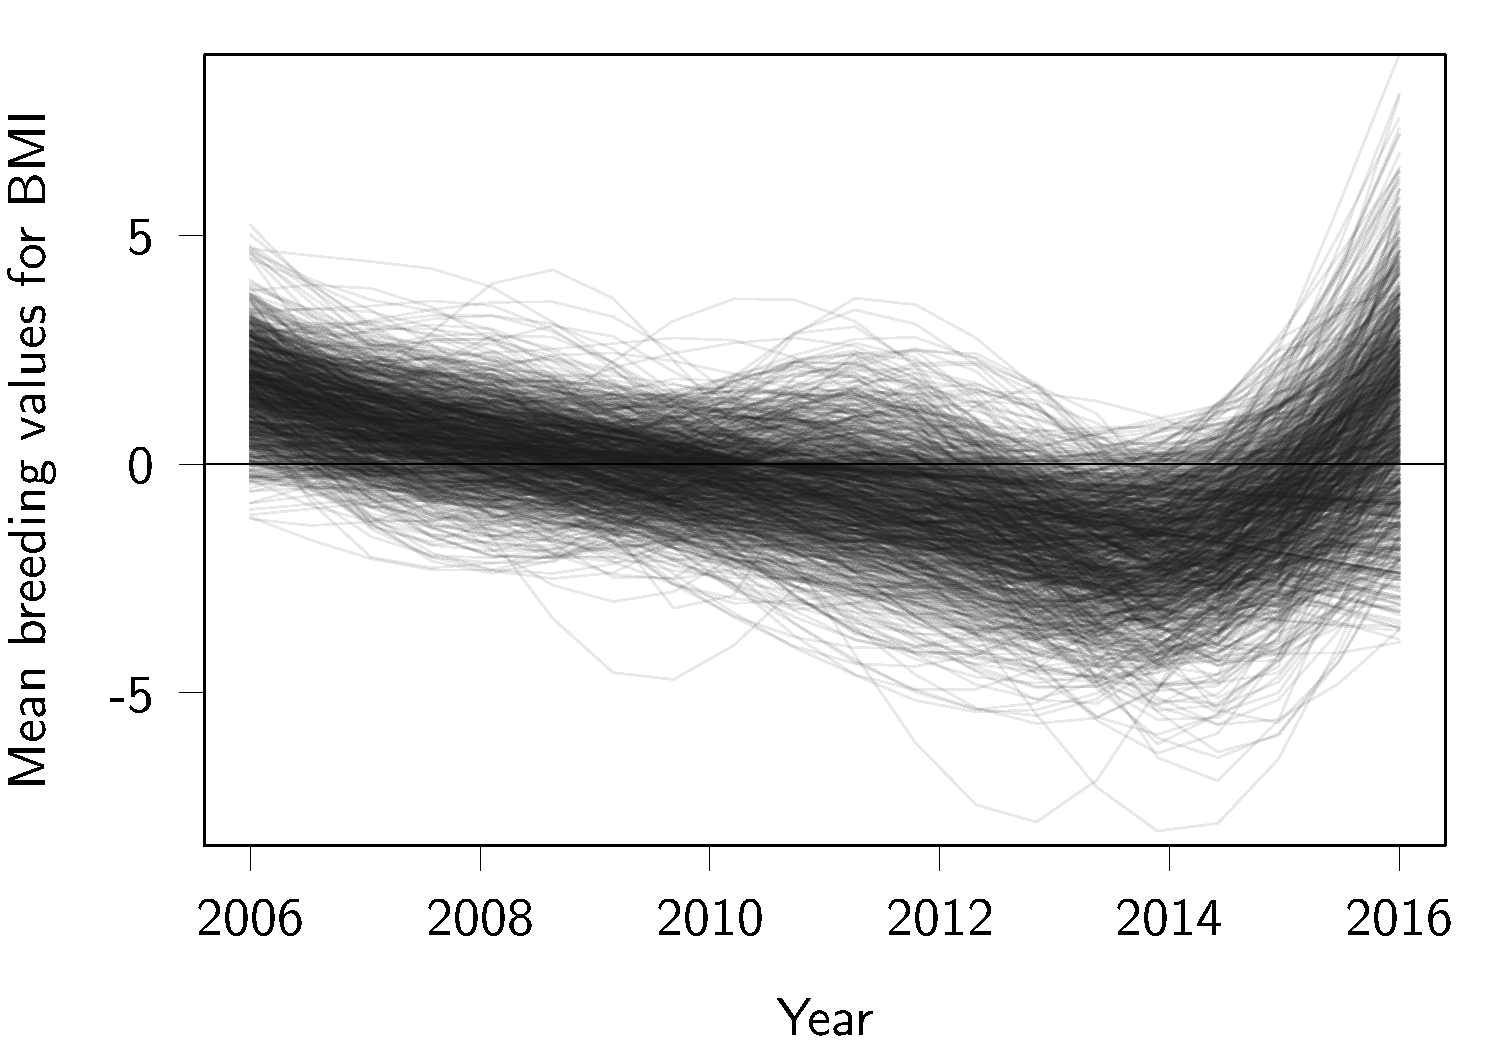
\includegraphics[width=\maxwidth]{figure/EvolSmooth-1} 

\end{knitrout}
\end{document}
